\chapter{Development}\label{chap:third chapter}

Since the implementation of the MPC algorithm is on a real system, and optimization is very computationally heavy, performing the computation on the ESP32 microcontroller was not the best way forward. Thus, communication was established between a host PC where all the heavy computation would take place and the microcontroller would be responsible for applying the calculated input and  measuring the states of the pendulum, followed by relaying this information to the host PC. A schematic of this setup can be found in Figure \ref{fig:Comms Schematic}.


\begin{figure}[htbp]
	\centering
	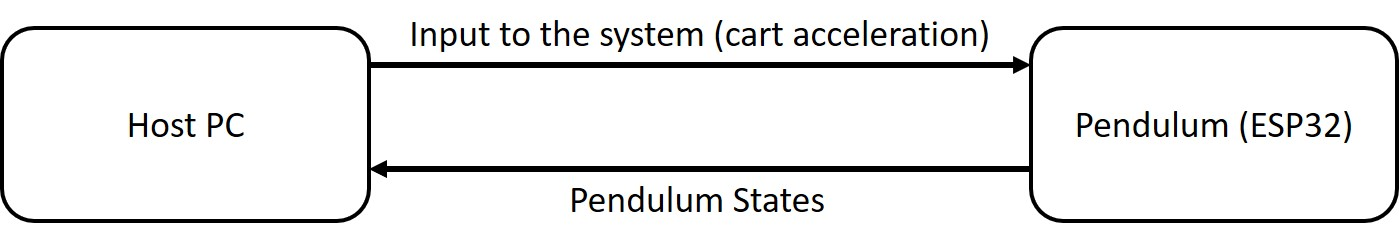
\includegraphics[width=\textwidth]{"src/Images/CommsSchematic.jpg"}   
	\caption{Concept Schematic}
	\label{fig:Comms Schematic}
\end{figure}

In this chapter we will take a look at both halves of this setup with a look into the MPC algorithm on the host PC side, the Arduino interface on the pendulum side and the established communication channel connecting the two halves.

\section{MPC}

As mentioned before, the first half of the system is the host PC where optimization is performed, with Python as the programming language of choice. For the purpose of easy access and understanding we encapsulated the parts into separate classes on python. 2 major tasks are carried out on the PC, namely : optimization and interfacing. In this section we will look at the optimization part in detail, with the interfacing being dealt with in further sections.

\subsection{Optimization on Python} \label{Section 3.1.1}

As suggested in Chapter \ref{Chapter 2}, the optimization problem uses a simple quadratic cost setup. The python script that performs the task of optimization is done with the help of the ACADOS package. ACADOS  is the successor of the ACADO software package developed at KU Leuven and University of Freiburg by the team of Prof. Moritz Diehl \cite{acados}.  

ACADOS offers extremely fast optimization time and makes it possible to run near the real time optimization requirement of the inverted pendulum. 

The state is measured and passed on to the $step()$ function that calculates the next controller step. The algorithm for which is as follows: 


\begin{algorithm}[H]
	\caption{MPC Control step}\label{alg:one}
	\KwData{$x_k$: Data at time step $k$ \\
		\hspace{1.3cm}Solver : a prebuilt ACADOS OCP solver object to be passed as an input to the \\ \hspace{2.5cm}$solve()$ function}
	\KwResult{$u$: Control input for time step $k+1$ }
	
	
	\eIf{first time = "True"}
	{
		initial guess for solver object $\gets$ first initial guess
	}
	%else
	{
		initial guess for solver object $\gets$ warm started initial guess
	}
	
	$x_{opt},u_{opt}$ $\gets$ Solve(solver,initial guess)
	
	$u$ $\gets$ $u_{opt}[0]$ \Comment{First Optimal Input} \\ 
	
	\textbf{Return} : $u$
	
\end{algorithm}

You are free to choose the first initial guess to the solver. Here, we load the solution of the first optimal control problem from a file as the first initial guess. 

As explained before, MPC involves using the first part of the optimal input trajectory to apply on the system. Although the rest of the sequence of inputs is not utilized, it can be reused in the next sampling instant to generate a rough estimate of optimal solution of the next QP problem. This technique is called warm-start and its primary reason is to reduce computational complexity in solving the next QP \cite{Otta2015}.


The optimization strategy used is sequential quadratic programming (SQP). This involves breaking down the problem into smaller quadratic program (QP)subproblems and optimizing each individual quadratic program \cite{Nocedal2006}.

These subproblems are solved using the partial condensing HPIPM(High Performance Interior Point Method). This involves the construction of a barrier function that is used to manage the inequality constraint \cite{Nocedal2006}.

Different solver options were tested and while the regular SQP method was far too slow in calculating the solutions, SQP with real time iterations ($SQP$\_$RTI$) \cite{acados,Diehl2005} was able to compute the solutions extremely fast due to a smaller local horizon . And in the interest of speed, the hessian, which is necessary for the calculation of optimal trajectories, is approximated using the Gauss-Newton approximation. This makes the problem more efficient. 

The optimization problem solved at every iteration is structured like the one described in previous chapters, which is as follows:
\begin{equation}
	\underset{\substack{x_0,x_1...x_N \\ u_0,u_1...u_{N-1}}} {\operatorname{min}} \sum_{k=0}^{N-1}\left (x_{k}^{T} Q x_{k}+ u_{k}^{T} R u_{k}\right)+x_{N}^{T} Q_f x_{N}^{T}
\end{equation}

\begin{equation}
	\begin{array}{ll}
		\text { subject to } & x_{k+1} = f(x_k,u_k)  \\
		& x_0 = x(0) \\
		
		& u_k \in \mathbb{U}, x_k \in \mathbb{X} \\
		
		& \forall k \in[0, N-1] \\
	\end{array}
\end{equation}

The values of $Q_k, R$ and $Q_f$ were tuned for optimal performance. The final values of these parameters are:

\begin{center}
	$Q_k = \begin{bmatrix}
		10 & 0       & 0      & 0      \\                       
		0  & 10^{-4} & 0      & 0      \\
		0  & 0       & 10^{4} & 0      \\
		0  & 0       & 0      & 10^{-2}\\
	\end{bmatrix}
	$
	\hspace{2cm}
	$R = \begin{bmatrix}
		10
	\end{bmatrix}
	$
\end{center}

$Q_f$ is decided by solving the infinite horizon LQR problem with the above mentioned $Q_k$ and $R$ values. This is common practice to achieve stability with MPC.


\section{Pendulum}

The pendulum is operated by the ESP32 microcontroller unit (MCU), a powerful and generic MCU with integrated Wi-Fi and Bluetooth connectivity for a wide range of applications \cite{ESPManual}

Since the ESP32 is an arduino peripheral one can use the arduino IDE to code instructions into the MCU. The ESP main $loop()$ function involves receiving, storing new data using the $recvWithEndMarker()$ and $storeNewData()$ functions. 
The algorithm for the main loop is as follows: 


\begin{algorithm}[H]
	\caption{Pendulum main loop}\label{alg:two}
	\KwData
	{	$x_k$: linear position data at time step k \\
		\hspace{1.4cm}$\theta_k$: angular position data at time step k \\
		\hspace{1.4cm}$dx_k$: linear velocity data at time step k \\
		\hspace{1.4cm}$d\theta_k$: angular velocity data at time step k \\
		\hspace{1.4cm}$u$ : received floating number of the input acceleration
	}
	
	\KwResult{$u_k$: The frequency needed to generate a desired linear velocity corresponding to the input signal.}
	
	
	
	\hspace{2mm}$u \gets read()$  \Comment{read() function reads a byte of serial data and stores it in an array} \\
	
	\hspace{2mm}$\theta_k \gets$ (PendulumEncoderPulses + 800) * 2$\pi$/1600 \\
	$x_k  \gets $ MotorEncoderPulses/20,000  \cite{PendulumManual} \\
	
	\eIf{current time - start time > 5ms}
	{
		$dx_k , d\theta_k \gets $ velocities calculated from measured valued of displacement 
	}
	{
		current time $\gets$ esp\_timer\_get\_time()  \Comment{ This line updates the current time variable}
	}
	
	sendStates($x_k, dx_k, \theta_k, d\theta_k$)      \Comment{Sends the states to the PC every 5ms}
	
	$u_k \gets$ real dynamics() \Comment {}
	
	start time $\gets$ current time    \Comment{This reassigns the start time as the current time}
	
	\textbf{Return} : $u_k$
	
\end{algorithm}
\clearpage


The $real$\_$dynamics()$ function calculates the value of the frequency of the PWM signal needed to generate the required velocity. The values of $x_k$ and $\theta_k$ values from the encoders of the pendulum. 

\begin{eqnarray}
	\theta_k= \frac{PendulumEncoderPulses+800)\cdot 2\pi}{1600} \\
	x_k =  \frac{MotorEncoderPulses}{20,000}
\end{eqnarray}


The encoder generates 400 pulses per revolution per channel. It has two channels, therefore, if the rising and falling edges are encountered, the resulting resolution is 1600 pulses per revolution. If we want to convert the pulses to angle in radians the simple math can be incorporated. And since we want the initial stable equilibrium position to correspond to an angle of $\pi$ radians, we add an additional 800 to the value of the rotary encoder pulses.
Similarly, the position can also be calculated by dividing the motor encoder pulses by a value of 20,000 \cite{PendulumManual}.






\section{Interfacing}

Now that we have established the 2 sides of communication channel, we can elaborate on the channel itself. In this section we will explain in detail the communication procedure on both the PC side and the microcontroller side.


\subsection{PC interface}

As mentioned before, python is the language used for optimization purposes and therefore is used to develop the PC interface of the communication channel as well. pySerial is a popular package for USB communication on Python and that is the package used in this particular application as well.

\textbf{Reading states from microcontroller:}

The Arduino has been programmed to continuously send the pendulum states every 5ms. To trigger the measurement of states on the PC side we use the $measure()$ function.

The read\_all() method in the serial module will read all the data that is available on the serial port and store it in a variable, this forms our buffer. We then extract the last 42 bytes from this buffer. With 4 states, one input and one delimiting character ("?") the total message size is 21 bytes. We extract the most recent 42 bytes in case of incomplete messages. 

The extracted message is then saved 4 bytes at a time to extract the 4 states. 


\textbf{Applying input:}

After calculating the input, $u$, as directed in section \ref{Section 3.1.1}, this input has to be applied to the pendulum cart. This can be done using the $apply()$ function on the PC side. This simply uses the $struct.pack()$ method to convert the input to its binary representation and $pySerial.write()$ function to send it to the pendulum via the connected serial port. 

\subsection{Pendulum interface}

As mentioned before, the pySerial package is used to establish a communication channel between the PC and the ESP32 microcontroller which controls the motor which in turns controls the pendulum. The ESP32 generates pulse width modulated (PWM) signals that cause motion in the stepper motor, generated by the LEDC peripheral on the EPS32, and thereby moving the pendulum cart.  \\


\textbf{Receiving from PC: the read() function}

The read function involves sequentially reading a byte of serial data and storing it in an array until the end of the message. This message is the input to the pendulum. The delimiter for this message is the $'\backslash n'$ symbol. 

\textbf{Sending to PC: real\_dynamics() and sendStates() functions}

The controller's output data is a sequence of four states, each of 4 bytes with the symbol,'?', denoting the start of this sequence.  To decrease the length of the message and increase the communication speed, the recorded floating point data was written as an address using IEEE754 standards instead of sending ASCII data of each number in the message. This is written into the serial buffer by the \textbf{sendStates()} function.

The \textbf{real\_dynamics()} function is responsible for the calculation of the frequency of the PWM signal from the received value of cart acceleration. This can be done using the following relation:

\begin{equation}
	f_{pwm} = v_{cart}\cdot20,000
\end{equation}

This relation comes from the formula for 

While calculating the frequency of the PWM signal, one has to account for the application of both high and low frequency signals. This can be done by adjusting the duty cycle resolution of the ESP32 clock.  Since frequency and duty resolution are inversely related one has to choose a resolution that can handle higher as well as lower frequencies. This can be done using the formula provided in \cite{ESPManual}. 

\begin{eqnarray}
	Duty  =\log_2 \left ( \frac{\mathit{f}_{clock}} {\mathit{f}_{pwm} * N_{clock}} \right)
	\\
	N_{clock} = \mathrm{A} + \frac{\mathrm{B}}{256}
\end{eqnarray}


Here $N_{clock}$ stands for the effective division factor of the arduino clock and the $\mathrm{A,B}$ here stand for the integer and fractional part of the division factor of the divider within the timer.  

From this one can calculate that for high velocities we require a duty resolution of 1-11 bits and for lower velocities we require a duty resolution of 8-20 bits. From this a resolution of 8 bits was chosen. In theory resolutions of 9,10 and 11 bits are also valid choices. 



